\chapter{Detalhes sobre a implementação do sistema} \label{sec:implementacao_sistema}

Nessa seção, apresentaremos detalhes técnicos sobre a implementação do sistema \textit{TomatoHealth}, tecnologias utilizadas e decisões do desenvolvimento tomadas para um sistema com as capacidades do descrito na seção \ref{sec:abst-det}.

\section{Arquitetura cliente-servidor e contêineres \emph{Docker}}

O \emph{TomatoHealth} implementa uma arquitetura de cliente-servidor, com dois tipos de clientes diferentes: clientes de usuários comuns e de especialistas, que se diferenciam conforme os requisitos das seções \ref{sec:abst-geral} e \ref{sec:abst-esp}.

Do ponto de vista da arquitetura cliente-servidor e da descrição abstratas para o usuário geral, os tópicos de mais difícil implementação são: tirar, enviar e receber uma foto para análise; já que entender o papel da ferramenta é uma tarefa do \emph{front-end}. Para realizar essas tarefas difíceis, o cliente faz uma requisição \emph{POST HTTP} enviando uma imagem com o uso da \emph{API FormData}\footnote{\url{https://developer.mozilla.org/en-US/docs/Web/API/FormData}}. E por sua vez, o servidor salva essa imagem no banco de dados \emph{S3 MinIO}, realiza a detecção das classes presentes, faz um prompt para a \emph{LLM} \texttt{gpt-4o-mini} da \emph{OpenAI} por \emph{API}\footnote{\url{https://platform.openai.com/docs/api-reference/introduction}} (pergunta ao modelo como tratar um tomateiro com as doenças detectadas) e finalmente responde o \emph{POST} do cliente com o \emph{output} da \emph{LLM}.

Já para o cliente especialista, as tarefas de ver as imagens tiradas por usuários comuns e demarcar as diferentes classes são solucionadas com a utilização da ferramenta de anotação \emph{Label Studio}. Essa ferramenta já incluí uma interface de rotulagem de dados que se comunica com o banco onde essas imagens são guardadas, e ela pode ser facilmente alterada para os propósitos da nossa aplicação.

Um modelo simples para nossa arquitetura pode ser visto na figura \ref{fig:modelo_arq}.

\begin{figure}[htbp]
    \centering
    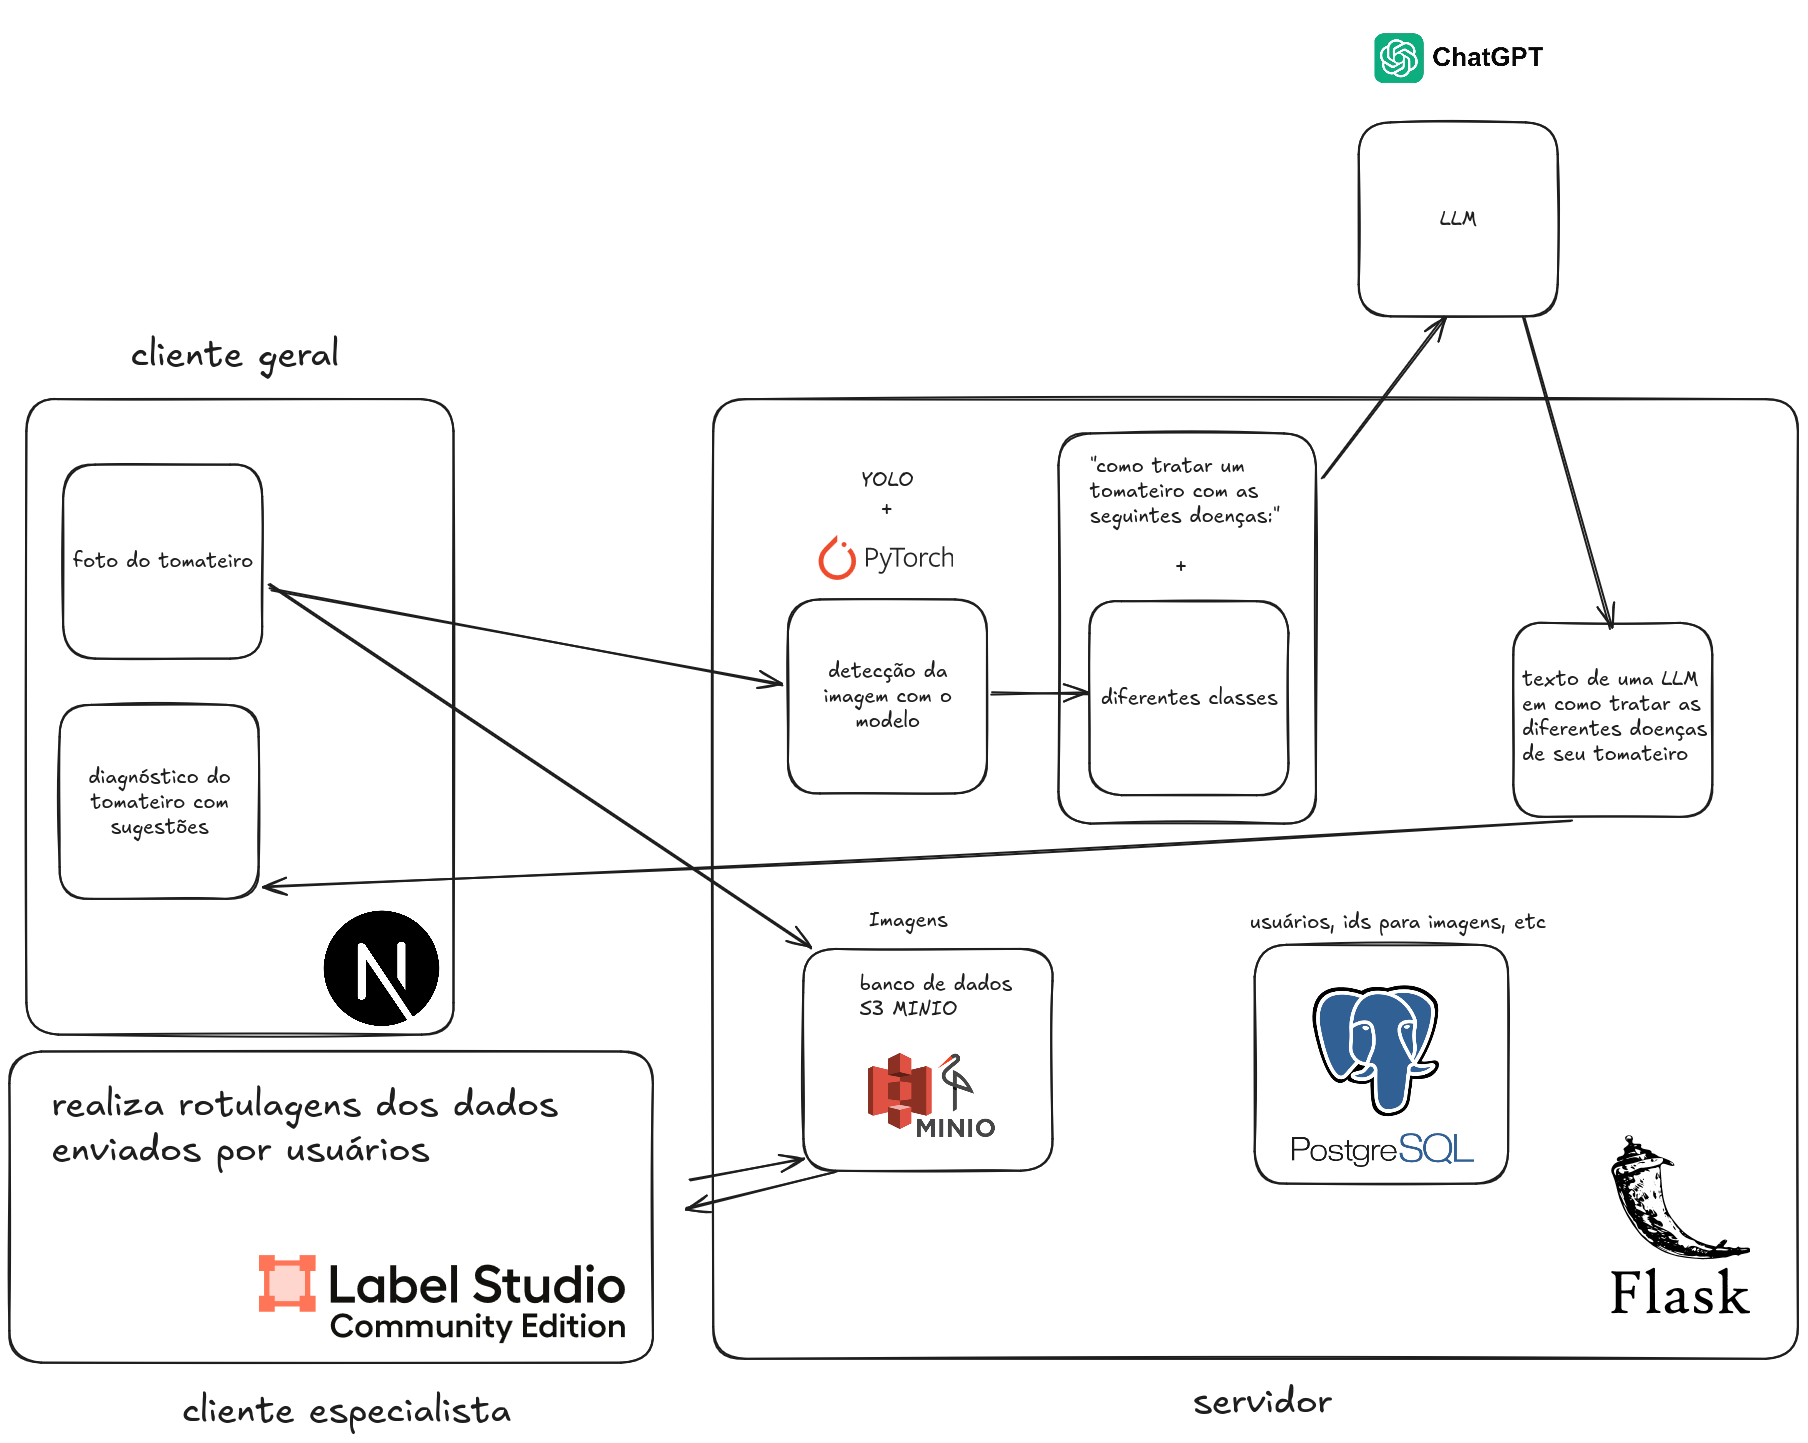
\includegraphics[width=1\linewidth]{images/modelo.png}
    \caption{\label{fig:modelo_arq} Modelo simples para a arquitetura implementada. A imagem apresenta as logos das tecnologias usadas: ChatGPT, Next.js, Label Studio, MinIO, PostgreSQL e Flask. Fonte: acervo dos autores.}
\end{figure}

Além disso, utilizamos contêineres \emph{Docker} \footnote{\url{https://www.docker.com/}}, pois facilitam o processo de desenvolvimento, uma vez que lidamos com o uso de diferentes \textit{frameworks} e bancos de dados, além de utilizarmos a ferramenta \emph{Docker Compose} para o controle de inicialização, execução e comunicação entre os contêineres. A figura \ref{fig:containers} demonstra os diferentes contêineres de nossa aplicação.

\begin{figure}[htbp]
    \centering
    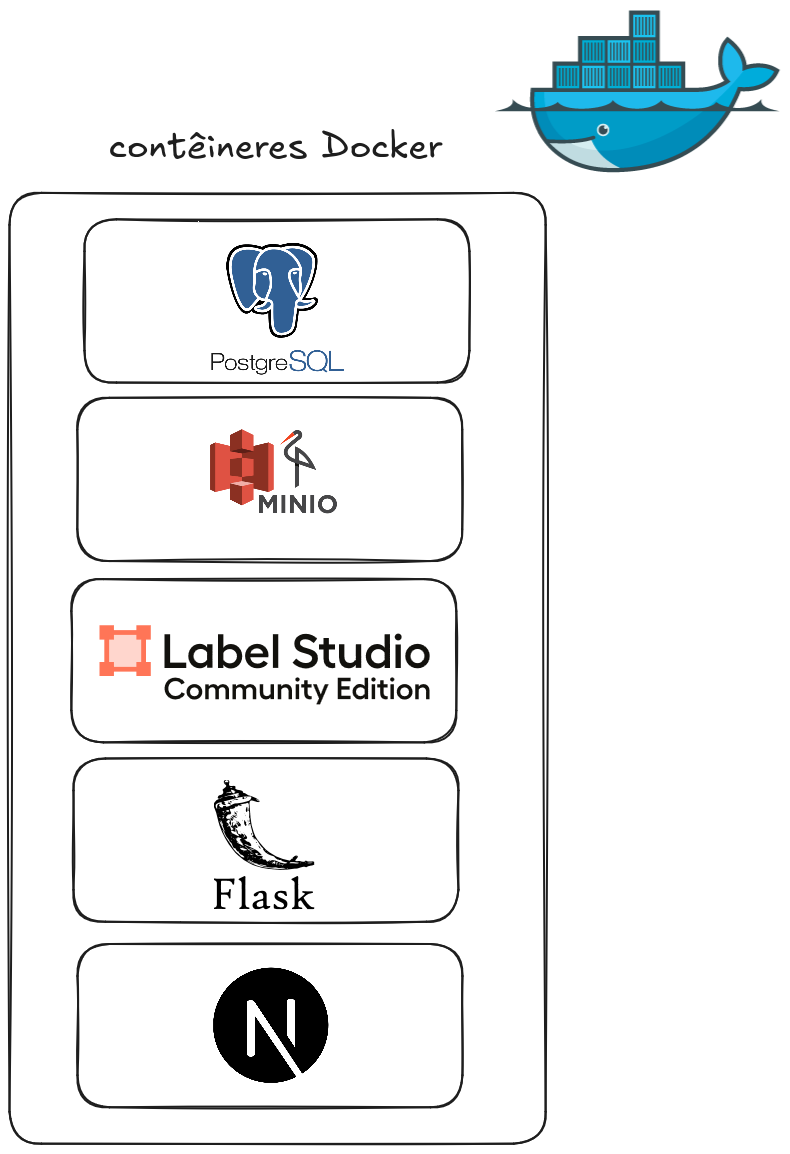
\includegraphics[height=0.5\textheight]{images/containers.png}
    \caption{\label{fig:containers} Modelo simples para os contêineres da nossa aplicação. A imagem apresenta as logos das tecnologias usadas: Docker, Next.js, Label Studio, MinIO, PostgreSQL e Flask. Fonte: acervo dos autores.}
\end{figure}

\section{\emph{Back-end}}
O \emph{back-end} do projeto foi implementado para contemplar os requisitos da seção \ref{sec:back-end-intro}. A maior parte do código foi feito utilizando \emph{Flask}\footnote{\url{https://flask.palletsprojects.com/en/stable/}}, um \emph{micro-framework Python} para aplicações \textit{web}.

Com essa ferramenta, implementamos os seguintes \emph{endpoints} principais (\emph{URL}s que representam funcionalidades no contexto da aplicação):
\begin{enumerate}
    \item \texttt{/process\_image}:
    \begin{enumerate}
        \item Recebe a imagem da folha do tomateiro enviada por um usuário regular;
        \item Obtém as respostas do modelo de detecção de objetos em relação às doenças presentes na imagem de folha do tomateiro:
        Isso é feito ao invocar o método de detecção de objetos do modelo de visão computacional (objeto em \emph{Python}) que é instanciado no início da aplicação
        \begin{lstlisting}
    # Run detection using YOLOv8
    detections = detection_model.predict(image, imgsz=640, conf=detection_threshold, device=device, verbose=False)
        \end{lstlisting}
        \item Salva a imagem enviada pelo usuário em um banco de dados de imagens:
        O banco de dados utilizado para a armazenagem de imagens é o \emph{S3 MinIO} \footnote{\url{https://min.io/}}, uma alternativa local ao sistema de armazenamento em nuvem \emph{S3} da AWS. Além de salvar as imagens enviadas pelos usuários, o \emph{MinIO} armazena todas as imagens do conjunto de dados em um diretório especial, no qual as imagens revisadas passarão a ser localizadas caso seja de interesse de um usuário administrador atualizar o conjunto de dados.
        \item Obtém a resposta de um modelo de linguagem que será entregue para o usuário:
        Utilizamos a \emph{API} da \emph{OpenAI}\footnote{\url{https://platform.openai.com/docs/overview}} para obter a resposta do modelo de linguagem;
        \item Envia a resposta à requisição;
    \end{enumerate}
    \item \texttt{/register\_admin}:
    Além do programa em \emph{Flask}, uma parte importante do \emph{back-end} da aplicação \emph{TomatoHealth} é um programa de linha de comando que oferece uma maneria simplificada dos administradores do sistema interagirem com ele. Com isso, é possível criar uma conta de administrador (que será registrada no banco de dados \emph{PostgreSQL}\footnote{\url{https://www.postgresql.org/}}. Com essa conta, temos acesso a todas as funcionalidades oferecidas pelo sistema, que serão explicadas a seguir.
    \item \texttt{/admin\_login}
    Depois de registrado um administrador, precisamos fazer \emph{login} na plataforma para receber um \emph{token} de autenticação \emph{JWT}. Isso é necessário pois as operações sensíveis, são protegidas.
    \item \texttt{/invite\_reviewer}
    Depois que um administrador está autenticado, ele pode convidar um usuário especialista para a plataforma. Isso é feito ao informar o \emph{e-mail} do especialista na requisição feita para \texttt{/invite\_reviewer}. Com isso, a ferramenta \emph{SendGrid} se encarrega de enviar um \emph{e-mail} convidando o usuário especialista a fazer parte da plataforma. 
    \item \texttt{/register\_reviewer/<token>}
    No \emph{e-mail} recebido pelo usuário especialista, há um link que leva para a página de registro. Essa página é renderizada pela aplicação \emph{Flask} ao acessarmos \texttt{/register\_reviewer/<token>} pelo navegador \emph{web}.
    \item \texttt{/login}
    Depois que o usuário especialista criou uma conta na plataforma, ele já pode efetuar o \emph{login}. Esse \emph{endpoint} também é renderizado pela aplicação e após um \emph{login} bem sucedido, o usuário especialista deve ser redirecionado para o endpoint \texttt{/labelling\_tool}.
    \item \texttt{/labelling\_tool}
    Nesse \emph{endpoint}, o usuário especialista será redirecionado para a plataforma de anotação das imagens enviadas pelos usuários. Então, é efetuada uma busca no banco de dados por imagens que ainda não foram revisadas. Ao encontrar uma imagem, uma tarefa no \emph{label-studio} é criada (revisão dessa imagem) e então o usuário especialista é redirecionado para essa tarefa, nesse momento, ele pode efetuar as revisões e, ao clicar no botão de finalizar a revisão, a imagem será marcada como revisada.
    \item \texttt{/update\_dataset}
    Em um momento que há diversas imagens marcadas como revisadas, um usuário administrador pode utilizar o \emph{endpoint} \texttt{/update\_dataset} para mover todas as imagens com o \emph{status} de revisadas para o diretório do \emph{MinIO} que contém o conjunto de dados inteiro.
    \item \texttt{/update\_weights}
    O processo de retreinamento do modelo (com a versão atualizada do conjunto de dados) será explicado a seguir. De qualquer maneira, um arquivo de pesos da rede neural é o resultado do treinamento e, para atualizar o modelo que está rodando na aplicação, basta enviar esse arquivo em uma requisição feita para o endpoint \texttt{/update\_weights}.
\end{enumerate}


\subsection{\emph{Machine Learning} no \emph{back-end} da aplicação}
\paragraph{Treinamento inicial:} antes de podermos iniciar a operação do sistema, seja em ambiente de desenvolvimento ou produção, um modelo de visão computacional é treinado para detectar as doenças dado uma imagem.

Após esse treinamento, obtemos um arquivo com a estrutura e os valores dos pesos do modelo treinado. Então, no programa \emph{Flask} do servidor, esse arquivo é usado para instanciar um objeto de rede neural (o modelo treinado). Assim, quando uma imagem é enviada via requisição para o endpoint \texttt{/process\_image}, obtemos os resultados das doenças detectadas pelo modelo nessa imagem ao invocar o método de inferência de seu objeto e usar a imagem recebida como argumento:
\begin{center}
\lstinline|detections = detection\_model.predict(image)|
\end{center}

\paragraph{Retreinamento:} para fazer o retreinamento do modelo de visão computacional, utilizamos o programa de linha de comando do administrador. Além disso, precisamos que o repositório do projeto esteja clonado na máquina responsável por esse processo (não só na máquina que roda a aplicação). Isso ocorre pois no repositório há um \emph{script Python} que faz o download do novo conjunto de dados do \emph{MinIO} e utiliza esses novos dados para treinar um novo modelo \emph{YOLO}. Ao final desse processo, o arquivo de pesos resultante é enviado automaticamente para o \emph{endpoint} \texttt{/update\_weights}. 

Uma funcionalidade interessante do projeto \emph{TomatoHealth} é a possibilidade de fazer o retreinamento do modelo de maneira remota (como por exemplo por meio de \emph{SSH}, isto é, acesso remoto). Para isso, um desafio importante que precisou ser superado é o fato de que precisaríamos de uma maneira de disponibilizar os dados do \emph{MinIO} e o \emph{endpoint} \texttt{/update\_weights} de alguma maneira que fosse acessível remotamente (do computador em que o retreinamento ocorre). Para isso, utilizamos a tecnologia de túnel de portas \emph{HTTP} da ferramenta \emph{Ngrok}\footnote{\url{https://ngrok.com/docs}}.


\paragraph{Uso do modelo de linguagem (\emph{LLM}):} depois de obtermos a classificação da condição das folhas identificadas na imagem, precisamos pensar em como entregar os resultados de uma maneira interessante para o usuário final.

Desse modo, implementamos uma integração dos resultados do modelo de detecção com a \emph{API} de modelos de linguagem da \emph{OpenAI}. Isso foi feito por meio da criação de um \emph{prompt} ao qual os resultados da tarefa de detecção de doenças é incorporado. Assim, o texto gerado pelo modelo de linguagem, que conterá informações sobre as doenças detectadas e dicas sobre como tratar a planta afetada é o retorno do \emph{endpoint} \texttt{/process\_image}. A estrutura do \emph{prompt} usado pode ser consultada a seguir. Note que há condições que mudam a estrutura do \emph{prompt}.

\begin{lstlisting}[literate={á}{{\'a}}1 {é}{{\'e}}1 {í}{{\'i}}1 {ó}{{\'o}}1 {ú}{{\'u}}1 {ç}{{\c{c}}}1 {ã}{{\~a}}1 {õ}{{\~o}}1]
Se nenhuma folha de tomate foi detectada:
"Não detectamos folhas de tomate na imagem."

Se apenas folhas saudáveis foram detectadas:
"De acordo com nosso algoritmo, seu tomateiro está saudável."

Caso contrário:
"A imagem de tamanho <image_width>x<image_height> pixels contém as seguintes doenças detectadas:

1. Doença: <class_name_1>
   Confiança: <score_1>
   Localização: De (<x1_1>, <y1_1>) até (<x2_1>, <y2_1>)

2. Doença: <class_name_2>
   Confiança: <score_2>
   Localização: De (<x1_2>, <y1_2>) até (<x2_2>, <y2_2>)

...

Por favor, providencie conselhos sobre como controlar e tratar as doenças detectadas e sugestões para melhorar o crescimento e a saúde da planta de tomate no geral."

Se ocorrer um erro na consulta ao modelo:
"Erro ao consultar o LLM: <mensagem_de_erro>"

\end{lstlisting}

\section{\emph{Front-end}}

\subsection{Cliente comum}

Para a interface de usuário geral, desenvolvemos duas páginas com a \textit{framework} \emph{React Next.js}, e utilizamos componentes da biblioteca \emph{React MUI}. As duas páginas são:

\begin{enumerate}
    \item página inicial
    \item página de diagnóstico do tomateiro
\end{enumerate}

Na primeira página, dividimos o site nas seguintes seções, como vistas na figura \ref{fig:homepage}, para o usuário conhecer o propósito da ferramenta e como a utilizar:

\begin{figure}[p]
    \centering
    \begin{subfigure}{0.45\textwidth}
        \centering
        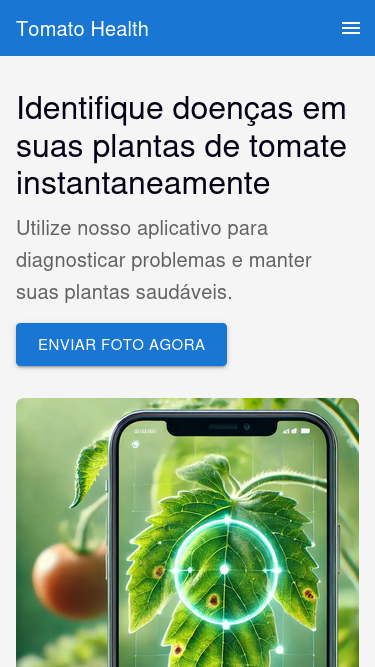
\includegraphics[width=\linewidth, height=0.4\textheight, keepaspectratio]{images/homepage1.png}
    \end{subfigure}
    \begin{subfigure}{0.45\textwidth}
        \centering
        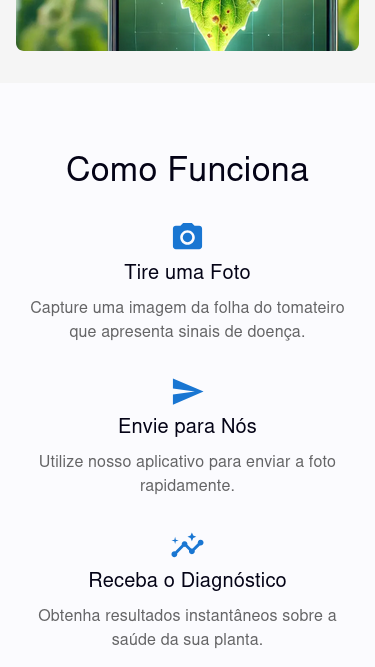
\includegraphics[width=\linewidth, height=0.4\textheight, keepaspectratio]{images/homepage2.png}
    \end{subfigure}
    
    \vspace{0.5cm}
    
    \begin{subfigure}{0.45\textwidth}
        \centering
        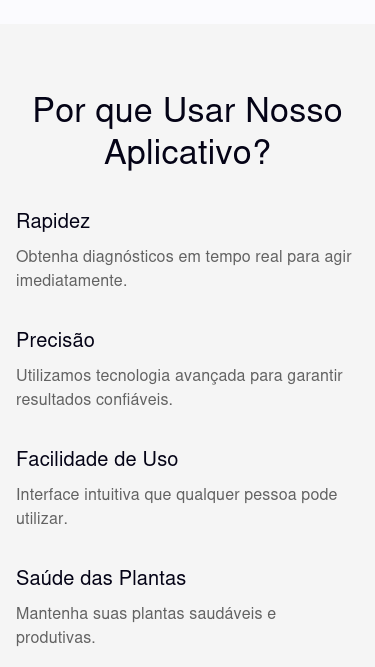
\includegraphics[width=\linewidth, height=0.4\textheight, keepaspectratio]{images/homepage3.png}
    \end{subfigure}
    \begin{subfigure}{0.45\textwidth}
        \centering
        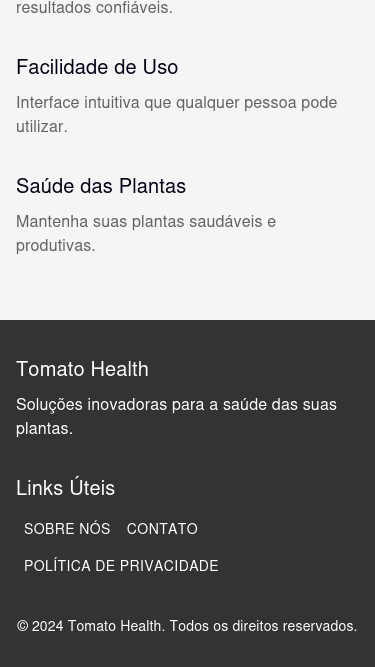
\includegraphics[width=\linewidth, height=0.4\textheight, keepaspectratio]{images/homepage4.png}
    \end{subfigure}
    
    \caption{Página inicial do TomatoHealth. Fonte da imagem utilizada: OpenAI, (2024), imagem gerada pelo modelo ChatGPT.}
    \label{fig:homepage}

\end{figure}

\begin{itemize}
    \item barra superior (\textit{app bar})
    \item destaque principal (\textit{hero section})
    \item \textit{call to action} (leva o usuário a diagnosticar sua planta)
    \item como funciona o \emph{TomatoHealth}
    \item por que usar nosso aplicativo
    \item rodapé
\end{itemize}

Na página de diagnóstico, como visto na figura \ref{fig:diagnostic}: o usuário escolhe tirar uma foto, ou então fazer \textit{upload} de sua galeria, para enviar ao servidor. O nosso \textit{front-end} então exibe a mensagem do servidor: o output de uma \emph{LLM}.

\begin{figure}[htp]
    \centering
    % Row 1
    \begin{subfigure}{0.3\textwidth}
        \centering
        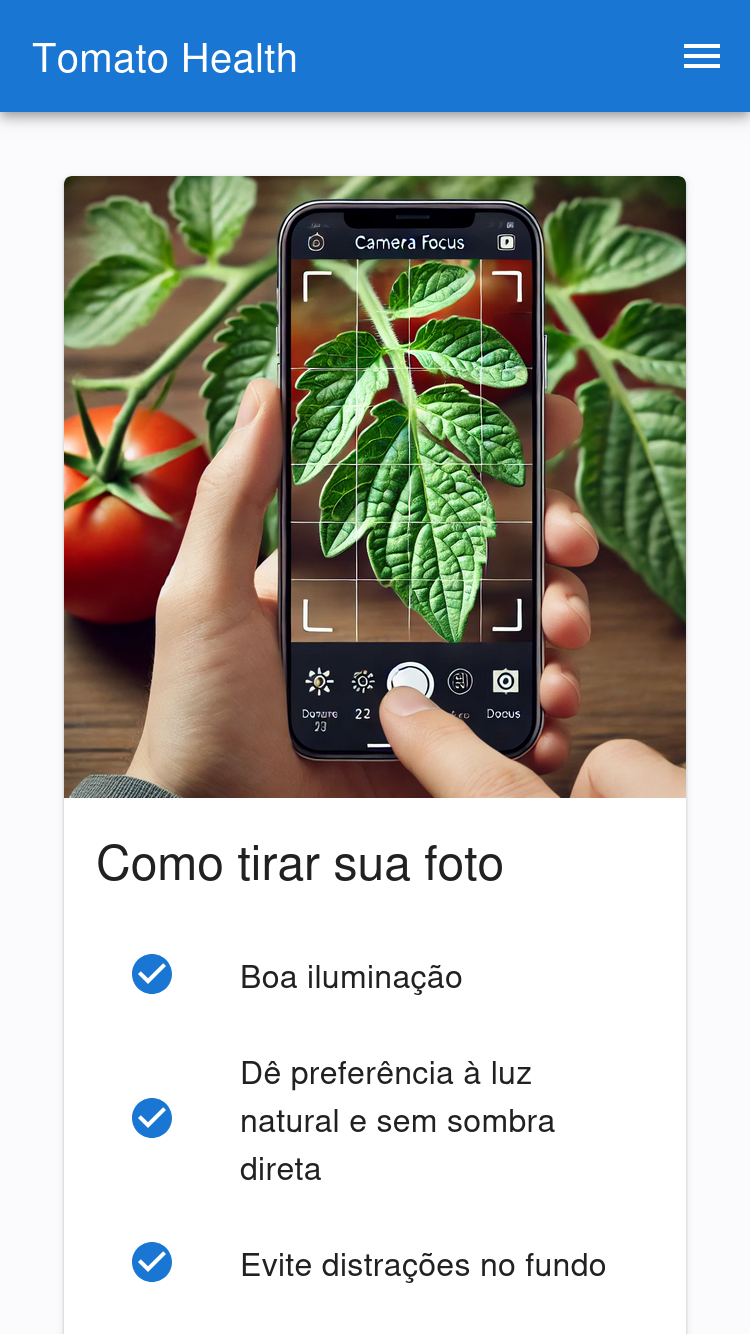
\includegraphics[width=\linewidth, height=0.4\textheight, keepaspectratio]{images/diagnostic1.png}
    \end{subfigure}
    \begin{subfigure}{0.3\textwidth}
        \centering
        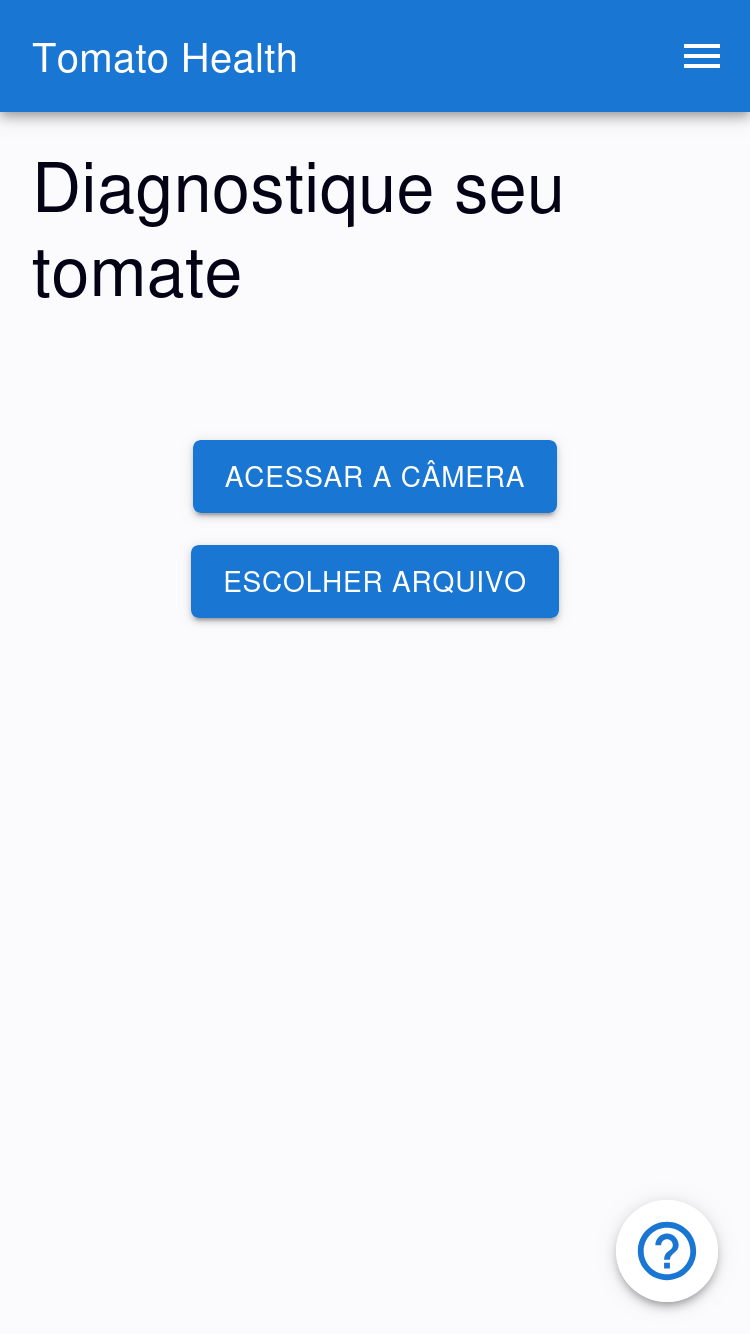
\includegraphics[width=\linewidth, height=0.4\textheight, keepaspectratio]{images/diagnostic3.png}
    \end{subfigure}
    \begin{subfigure}{0.3\textwidth}
        \centering
        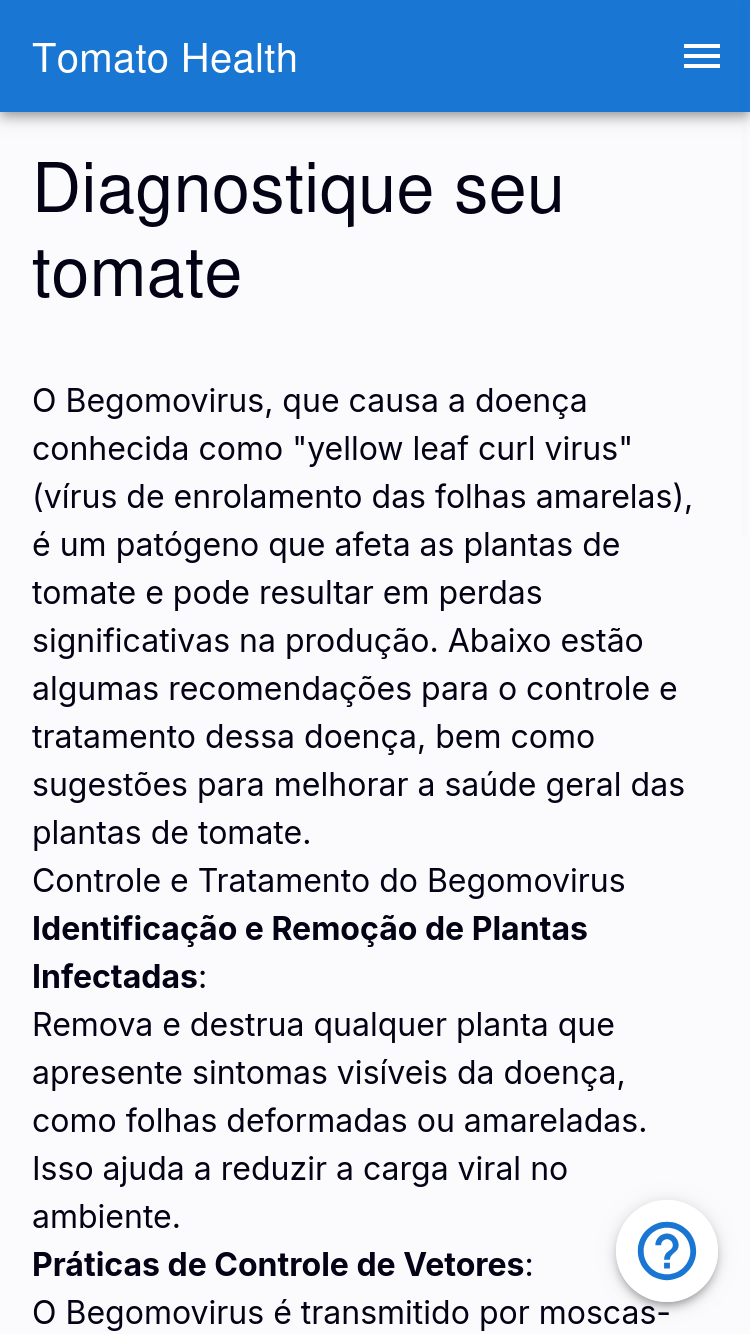
\includegraphics[width=\linewidth, height=0.4\textheight, keepaspectratio]{images/diagnostic5.png}
    \end{subfigure}
    
    % Add spacing between rows
    \vspace{0.5cm}
    
    % Row 2
    \begin{subfigure}{0.3\textwidth}
        \centering
        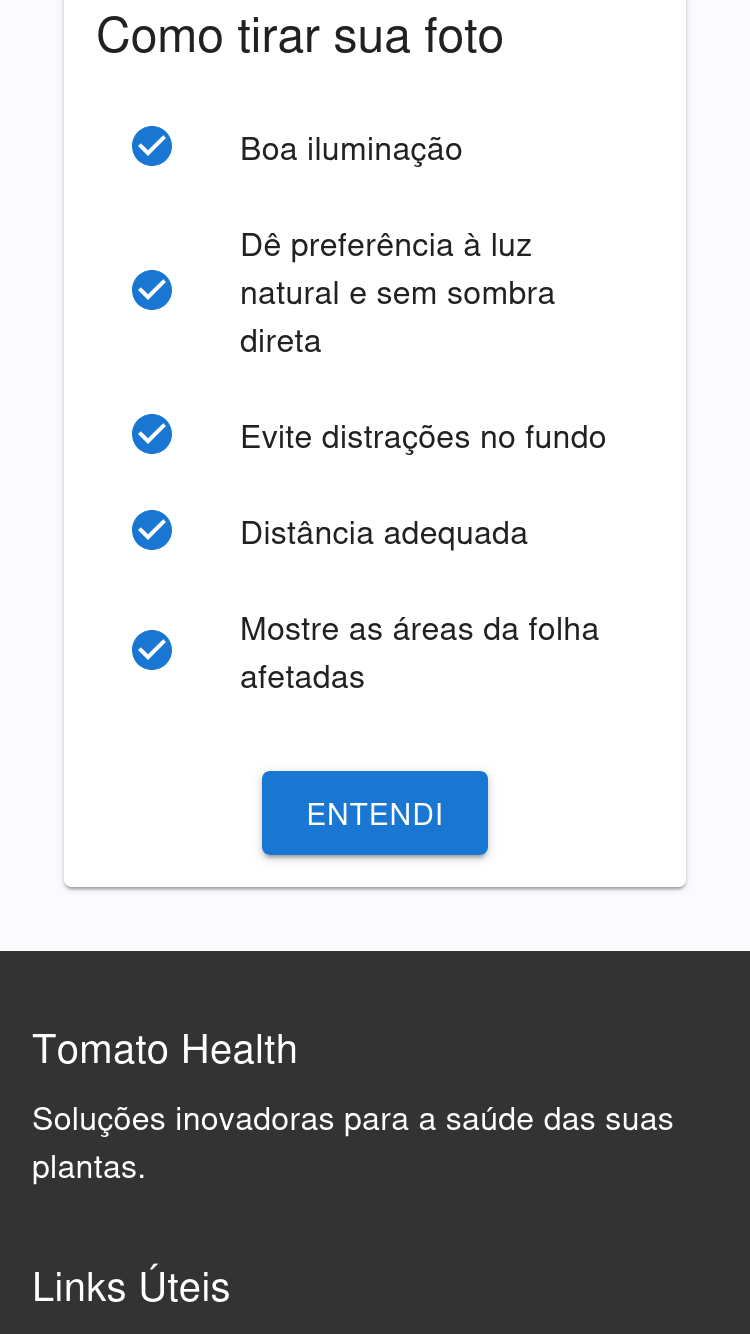
\includegraphics[width=\linewidth, height=0.4\textheight, keepaspectratio]{images/diagnostic2.png}
    \end{subfigure}
    \begin{subfigure}{0.3\textwidth}
        \centering
        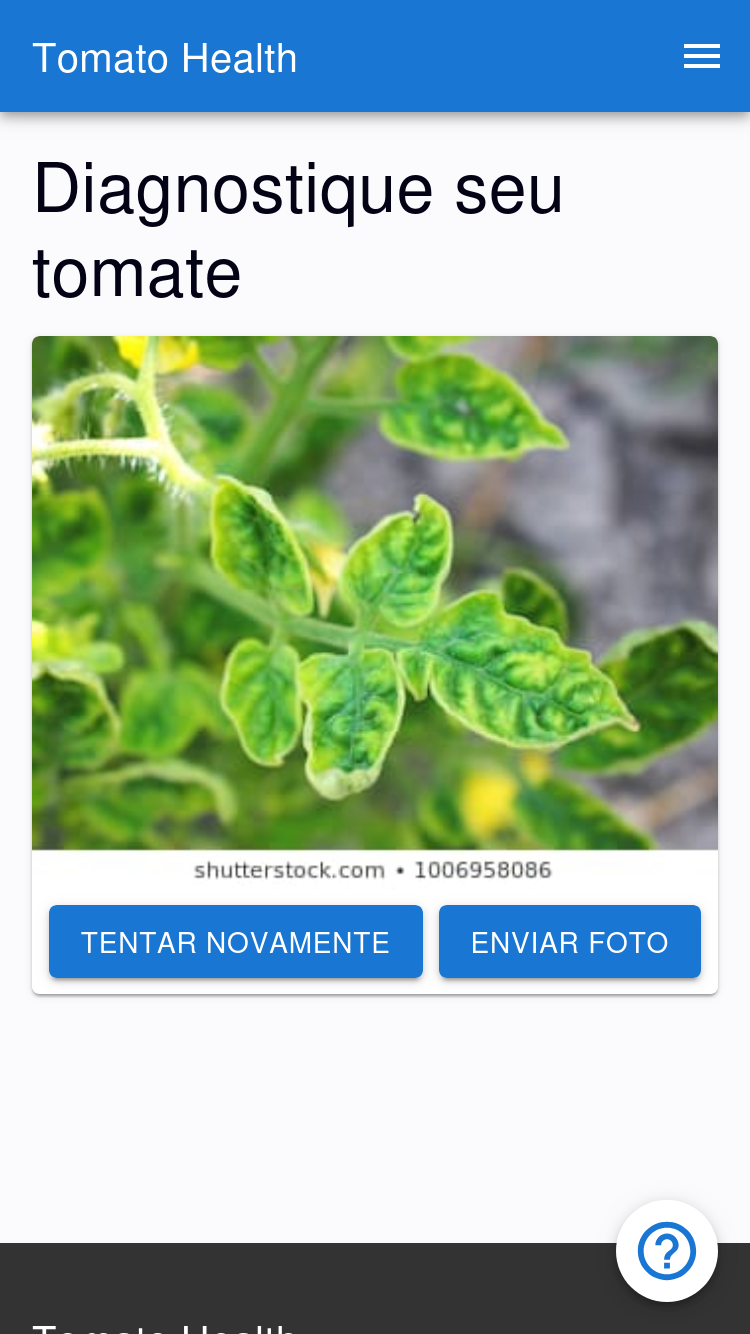
\includegraphics[width=\linewidth, height=0.4\textheight, keepaspectratio]{images/diagnostic4.png}
    \end{subfigure}
    \begin{subfigure}{0.3\textwidth}
        \centering
        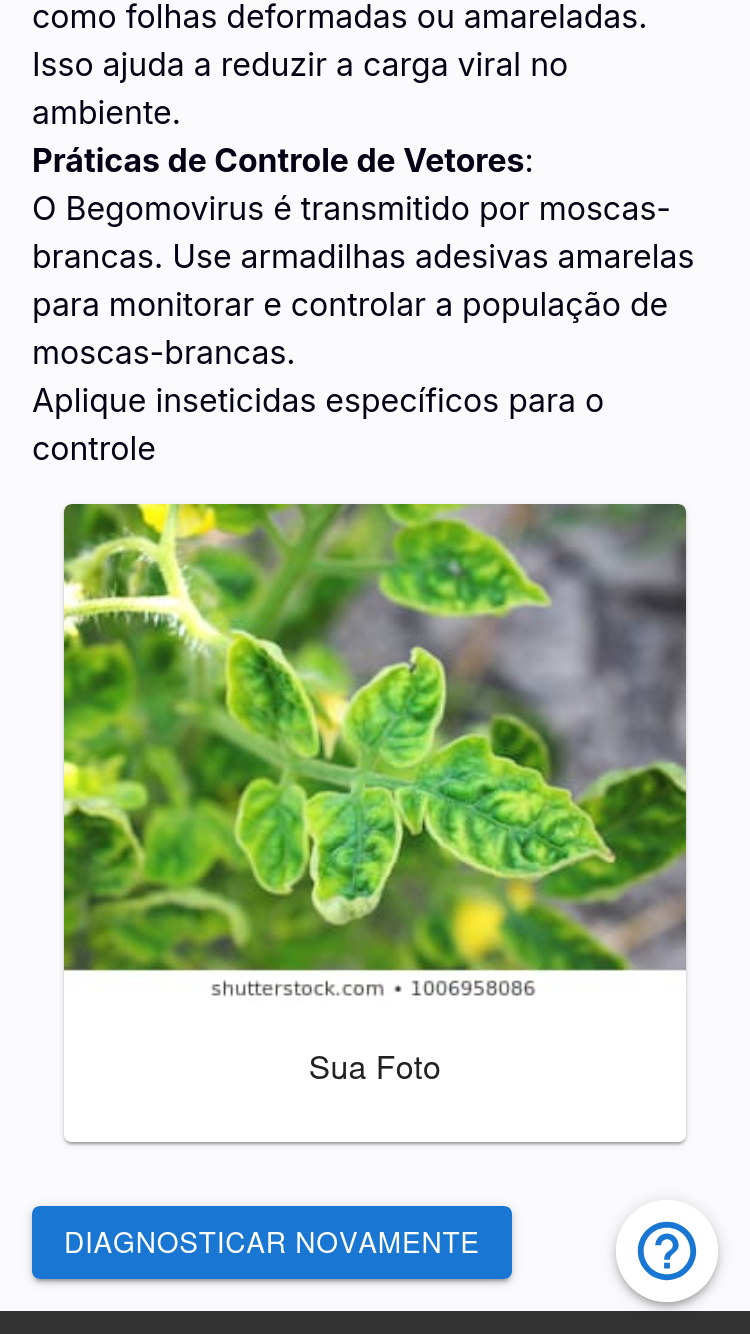
\includegraphics[width=\linewidth, height=0.4\textheight, keepaspectratio]{images/diagnostic6.png}
    \end{subfigure}
    
    \caption{Página de diagnóstico do TomatoHealth. Fonte da imagem utilizada: OpenAI, (2024), imagem gerada pelo modelo ChatGPT.}        
    \label{fig:diagnostic}
\end{figure}


\subsection{Cliente especialista e ferramenta de anotação \emph{Label Studio}}

Na interface do usuário especialista, utilizamos o \textit{software open-source} de rotulagem \emph{Label Studio}. Segundo sua página no \emph{Github}, "O Label Studio é uma ferramenta de rotulagem de dados de código aberto. Ela permite rotular tipos de dados como áudio, texto, imagens, vídeos e séries temporais com uma interface de usuário simples e direta e exportar para vários formatos de modelos. Ele pode ser usado para preparar dados brutos ou melhorar os dados de treinamento existentes para obter modelos de ML mais precisos".

Para não exibir detalhes desnecessários do sistema, modificamos seu código \textit{front-end} em \emph{React}, de forma a excluir alguns componentes da página de anotação, como barras nas laterais e no topo da página, com a finalidade do usuário não visitar endereços não utilizadas pelo \emph{TomatoHealth}.

Conforme a figura \ref{fig:rotulagem_labelstudio}, o usuário especialista vê, por vez, uma única imagem que ele poderá demarcar classes de doenças com \textit{bounding boxes}. Após ele efetuar a rotulagem, o banco de dados é atualizado com as novas informações e o usuário é redirecionado para a próxima imagem.

\begin{figure}[htbp]
    \centering
    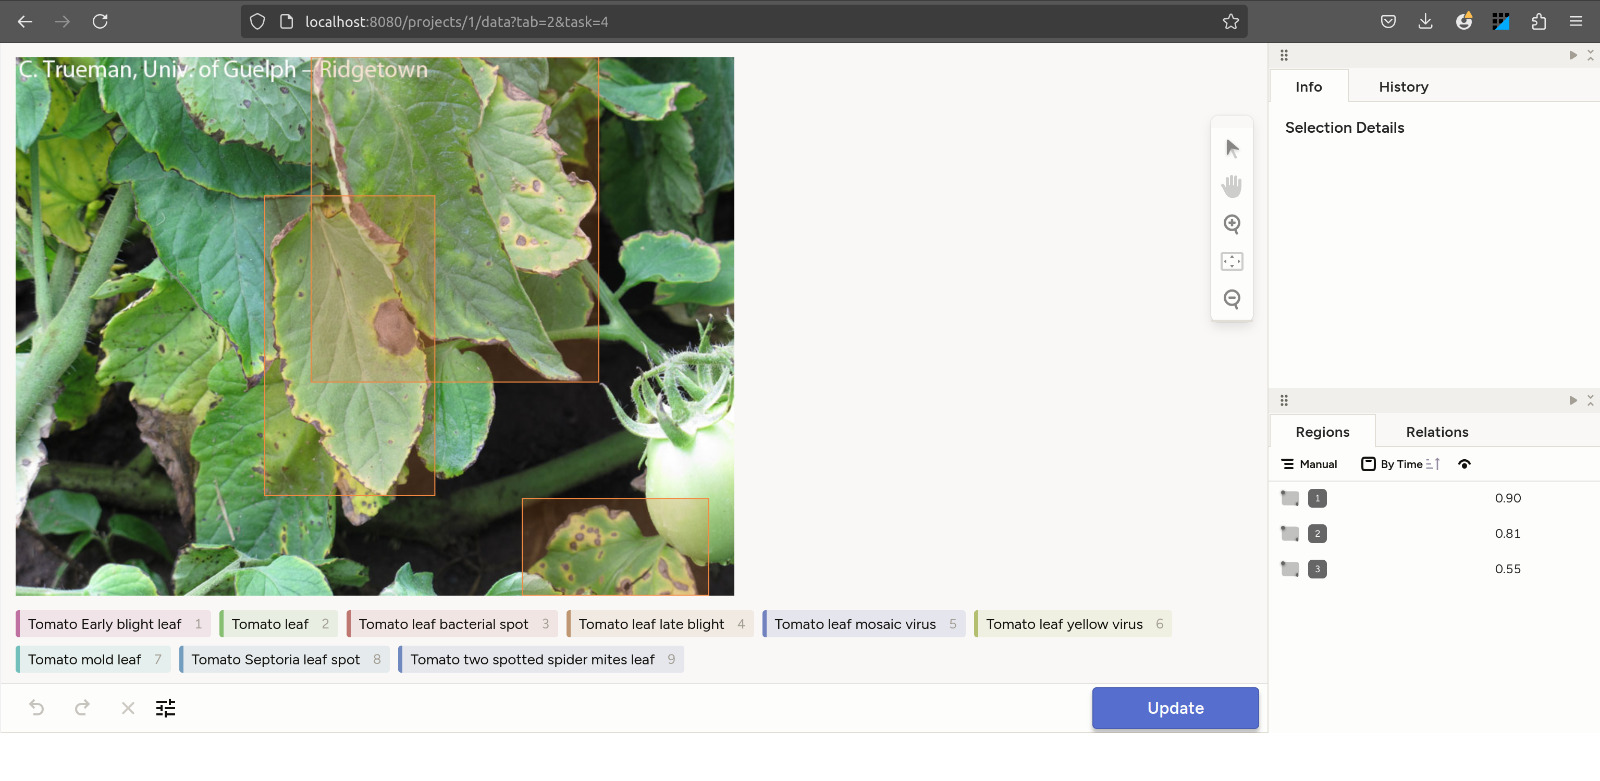
\includegraphics[width=1\linewidth]{images/rotulagem_labelstudio.jpg}
    \caption{\label{fig:rotulagem_labelstudio} Página de rotulagem do usuário especialista utilizando uma versão modificada do Label Studio. Fonte: acervo dos autores.}
\end{figure}